\chapter{شیوه پژوهش‌}
با بررسی برخی مفاهیم کلی در فصل پیشین، اطلاعات اولیه به منظور علاقه‌مندی به موضوع و همچنین پیش‌زمینه مورد نیاز برای ادامه فراهم شد و در این فصل کمی درباره متدلوژی تحقیقاتی و روش پژوهشی که در این پروژه استفاده شده است، صحبت خواهیم کرد.\\
در ابتدای پژوهش و با کسب دانش ‌زمینه مورد نیاز، به جستجوی پراکنده پرداختیم و برخی تعاریف و مفاهیم را از منابع مختلفی که در بخش مراجع ذکر شده‌اند استخراج کردیم اما به منظور انجام این پژوهش، نیازمند یک روش ساختارمند و مشخص در تحقیق بودیم که بتوانیم استدلال قوی‌تر و نتیجه‌گیری موثق‌تری داشته باشیم.
\begin{figure}
	\centering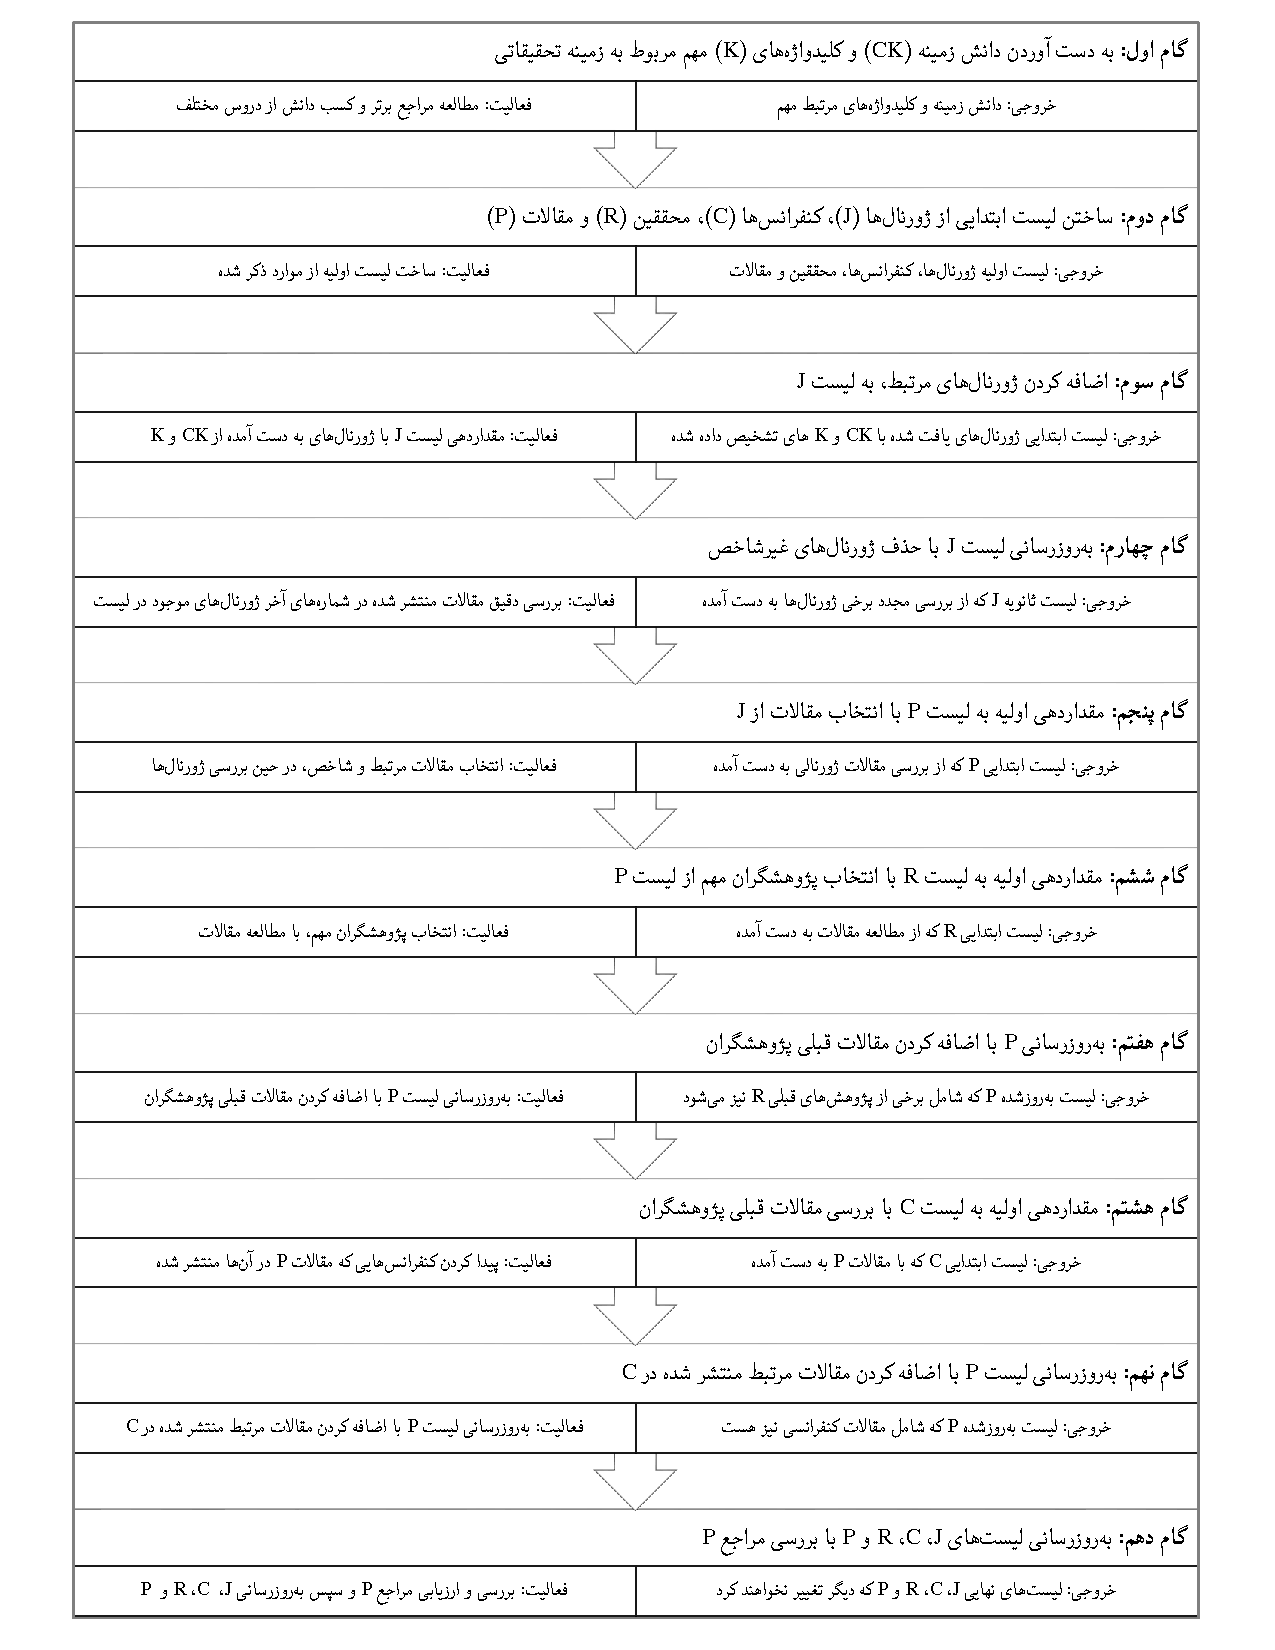
\includegraphics[width=\linewidth]{Resources/ISLAB_methodology.pdf}
	\caption[متدلوژی پژوهشی آزمایشگاه سیستم‌های هوشمند و گام‌های آن]
	{متدلوژی پژوهشی آزمایشگاه سیستم‌های هوشمند و گام‌های آن؛ گام‌های این متدلوژی پایه و اساس این پژوهش را ساخته‌اند که مراحل آن در تصویر قابل مشاهده است. گام‌های متدلوژی را تا جایی ادامه می‌دهیم که منابع کافی برای انجام پژوهش را داشته باشیم.}
	\label{fig:islab}
\end{figure}
به عبارتی دیگر برای انجام این پژوهش، می‌بایست ژورنال‌ها
(\lr{J})،
کنفرانس‌ها
(\lr{C})،
محققین‌
(\lr{R})
و مقاله‌های (\lr{P}) مرتبط و موثر را شناسایی کنیم.\\
با رجوع به شیوه پژوهش آزمایشگاه سیستم‌های هوشمند\LTRfootnote{ISLAB Research Methodology}
که یکی از  شیوه‌های پژوهش موثر در مطالعات و پژوهش‌های موردی، در حال استفاده توسط پژوهشگران این آزمایشگاه است، درمی‌یابیم که می‌بایست در چند تکرار و به صورت تکاملی منابع مورد نیاز برای پژوهش خود را آماده سازیم.\\
بدین منظور،‌  مطابق  شکل 
\ref{fig:islab}
ابتدا به جمع‌آوری دانش موضوعی\LTRfootnote{Context Knowledge}
(\lr{CK}) در زمینه مورد نظر پرداختیم و سپس شروع به یافتن کلیدواژه‌های مطرح (\lr{K}) در این زمینه نحقیقاتی کردیم؛ از جمله این فعالیت‌ها می‌توان به مطالعه منابعی چون
\cite{albert_measuring_2013}، \cite{pressman_software_2015}، \cite{p._miguel_review_2014} و \cite{sommerville_software_2016}
و همچنین اخذ درس‌هایی مانند مهندسی نرم‌افزار نام برد (گام اول).
\begin{table}[H]
	\caption[کلیدواژه‌های به دست آمده از دانش زمینه]{
		کلیدواژه‌های به دست آمده از دانش زمینه؛ با استفاده از دانش زمینه، کلیدواژه‌هایی را فرا آموختیم که از طریق آنان منابع مربوط به پژوهش خود را به دست آوریم.
	}
	\label{tab:keywords}
	\centering\begin{tabular}{|c|c|}
		\hline
\textbf{ردیف} & \textbf{کلیدواژه}         \\ \hline
		۱    & \lr{Business Data Processing}  \\ \hline
		۲    & \lr{Crowd}                     \\ \hline
		۳    & \lr{Crowdsourcing}             \\ \hline
		۴    & \lr{Crowdsourced Data Cleaning}             \\ \hline
		۵    & \lr{Interaction}               \\ \hline
		۶    & \lr{Online Experiment}         \\ \hline
		۷    & \lr{Software Quality}          \\ \hline
		۸    & \lr{Usability}                 \\ \hline
		۹    & \lr{Usability Evaluation} \\ \hline
		۱۰    & \lr{Usability Quality Metrics} \\ \hline
		۱۱   & \lr{Usability Study}           \\ \hline
		۱۲   & \lr{Usablity Quality Model}    \\ \hline
		۱۳   & \lr{User Experience}           \\ \hline
		۱۴   & \lr{User Interface}            \\ \hline
		۱۵   & \lr{Web Usability}          \\ \hline
	\end{tabular}
\end{table}
سپس، چند لیست تهی برای ذخیره اطلاعات ژورنال‌ها، کنفرانس‌ها، پژوهشگران و همچنین مقالات مختلف مرتبط و موثر در این حوزه تحقیقاتی ساختیم، که به‌طور خلاصه با حروف
\lr{J}، \lr{C}، \lr{R} و \lr{P}
از آن‌ها یاد می‌کنیم (گام دوم).\\
با استفاده از دانش زمینه به دست آمده و همچنین کلیدواژه‌های شناخته شده که گزیده‌ای از آن‌ها در جدول 
\ref{tab:keywords}
قابل مشاهده است، لیست‌های
\lr{J}، \lr{C}، \lr{R} و \lr{P}
را به طور مرتب و با تکرارهای متعدد، به‌روزرسانی کردیم (گام‌های سوم تا دهم) تا اینکه به منابع ذکر شده در این سند
%\ref{tab:confs}
%\ref{journals}
%\ref{papers}
%\ref{researchers}
رسیدیم و منابع مورد نیاز پژوهش را، تا جایی که بتوان به نتیجه قابل اتکایی رسید، با این متدولوژی پژوهشی و با استفاده از ابزارهایی چون
\cite{noauthor_computing_nodate}
و 
\cite{noauthor_dblp:_nodate}
و نیز
\cite{noauthor_scimago_nodate}
پیدا کردیم. پس از شناخت دامنه و به دست آوردن منابع لازم، یک تعریف نیازمندی برای ابزار تست مورد نظر ارائه دادیم که بر اساس آن سیستم هدف و ابزار مطرح در این پژوهش ساخته شد.